\documentclass{deltares_manual}

\usepackage{tikz}
\usepackage[pipeTables=true]{markdown}

%------------------------------------------------------------------------------
\newcommand{\dfastbe}{\textrm{D-FAST~Bank~Erosion}\xspace}

\hypersetup
{
    pdfauthor   = {Deltares},
    pdftitle    = {\dfastbe},
    pdfkeywords = {Technical Reference \dfastbe}
}

%------------------------------------------------------------------------------
%

%\makeindex

%------------------------------------------------------------------------------
%
\begin{document}
%\pagestyle{empty}
%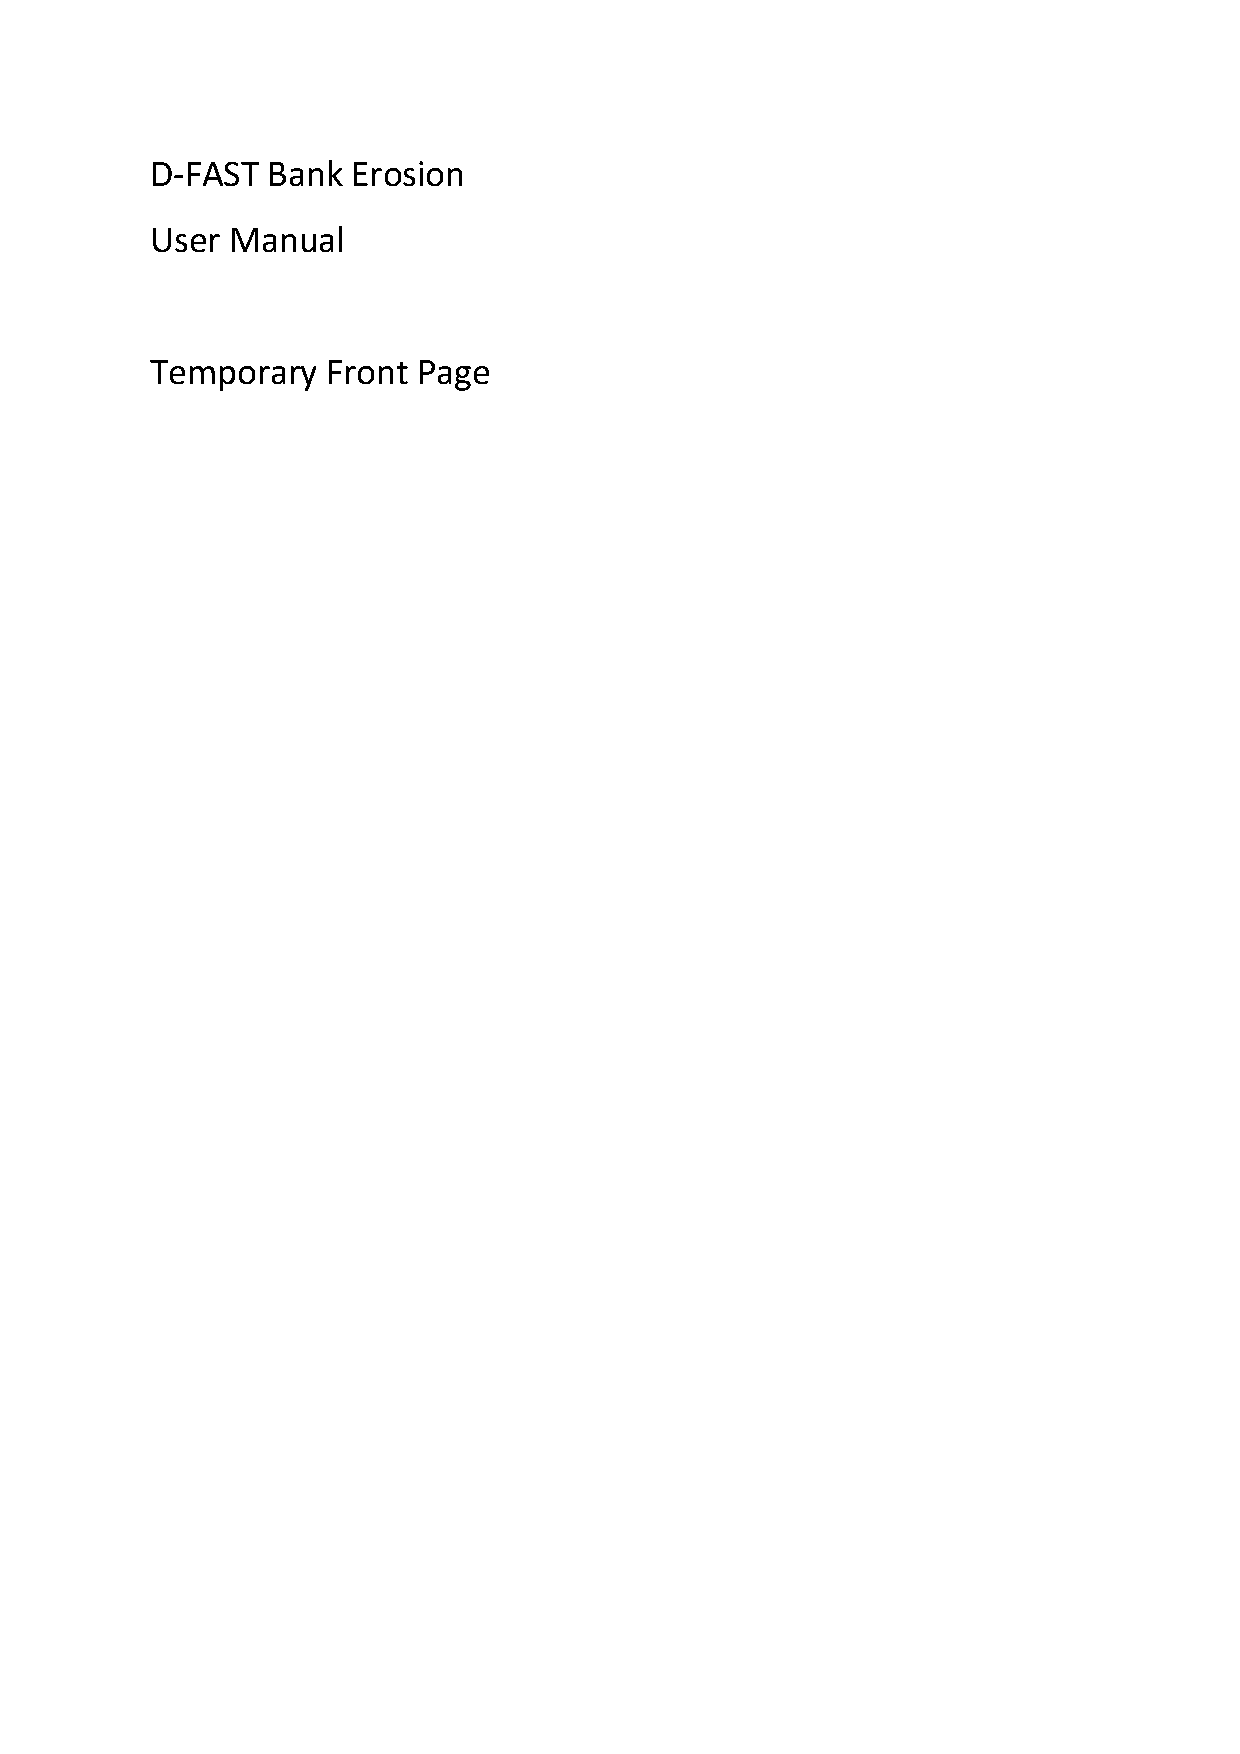
\includepdf[pages=1, offset=72 -70]{cover/d-fast-bank-erosion.pdf} % links-rechts past precies
%\cleardoublepage
\title{D-FAST\\ Bank Erosion}
\subtitle{}
\manualtype{Technical Reference Manual}
\version{1.0}

\author{Bert Jagers}

\deltarestitle
%
\chapter{Introduction}

This document describes the code design considerations for the development of \dfastbe.
\dfastbe is the successor of WAQBANK.
The purpose of these tools is to provide an estimate of the bank erosion due to currents and shipping.
The conceptual WAQBANK framework was developed since 2010.
To obtain the estimate of the bank erosion, the algorithm needs data on e.g.

\begin{itemize}
\item velocity distribution at a number of representative discharges,
\item bank composition and protection, and
\item shipping characteristics.
\end{itemize}

Based on these data the algorithm provides estimates of the average and maximum erosion distances along the studied reach after a characteristic period, and when the ultimate equilibrium conditions have been reached.
The original WAQBANK tool performs the analysis based on results obtained from WAQUA or Delft3D 4 simulations.
The new \dfastbe tool performs the analysis based on D-Flow FM simulation results.
%\chapter{Detecting and shifting the bank lines} \label{Chp:BankDetect}

This chapter describes the algorithms used for detecting (see \autoref{Sec:BankDetect}) and shifting (see \autoref{Sec:BankShift}) the bank lines.
The former happens in the 'banklines' detection step, whereas the latter happens in the 'bankerosion' analysis step after the bank erosion rates have been computed.
It also lists issues that you may run into during the detection step (see \autoref{Sec:DetectIssues}).

\section{Detecting the bank lines} \label{Sec:BankDetect}

The location of bank lines is determined by identifying the boundary between water (wet) and land (dry) at a reference discharge computed using \dflowfm.
The detection of the bank lines builds on the search lines provided as input to this step.
The model domain is first clipped to the area close to the search lines (i.e.~within the user specified search distance from the search line) to focus the bank detection algorithm on the areas of interest only.
Identifying the exact location of the bank lines starts by determining for each grid cell in the area of interest whether it has one (or more) bed levels $z_b$ (defined at the mesh nodes) above the water level $z_w$ in the grid cell and one (or more) bed levels below the water level (see \autoref{Fig:detect_step}).

\NumNote{\dfastbe currently only supports results of hydrodynamic simulations which use bed levels $z_b$ defined at grid nodes.
Simulations with bed levels defined in cell centres (tile depth) are thus not supported.}

\begin{figure}[!h]
\center
\resizebox{5cm}{!}{
   \input{figures/detect_step.pdf_tex}
}
\caption{The bank line determined by the transition from wet (bed levels $z_b$ below water level $z_w$) to dry (bed levels $z_b$ above water level $z_w$) per triangle}
\label{Fig:detect_step}
\end{figure}

For each of those grid cells, the sub-grid boundary between dry and wet parts is determined as the line along which the interpolated bed level equals the water level in the grid cell.
The line marking the zero water depth is a straight line in a triangle.
Cells with $N_c \ge 4$ corners are split into $N_c - 2$ triangles to arrive at a collection of only straight line segments.
The collection of all these line segments forms the basis of the final bank line, which is obtained by connecting the individual segments into long connected strands.
Subsequently, those bank line strands are selected that are closest to the river axis (to avoid selecting banks of floodplain lakes or side channels that are located close to the bank of interest).
The selected strands are finally connected across side channels entrances and other gaps to a continuous bank line for the whole reach of interest.
The resulting lines are written to a shape file for checking and use in the 'bankerosion' analysis step.

The found locations of the bank lines will clearly depend on the chosen discharge level.
However, as long as the discharge is within the main channel, the locations will be fairly consistent.

Generally, bank erosion only occurs along the main channel.
It is therefore possible to only take into account those cells that are within a certain distance from the predefined search lines.
This is also necessary when more than one bank line is present (as is common in rivers), because otherwise it is not clear which coordinates belong to one bank or the other.

The search lines should be defined in a simple text file consisting of x- and y- coordinates (\command{Line1}, ..., \command{LineN}, in the configuration file).
For the Dutch rivers the lines can be obtained from the Baseline 'oeverlijnen' for model schematisations up to Baseline 4.
For model schematisations of Baseline 5 and higher the 'oeverlijnen' can be obtained by:
%
\begin{enumerate}
\item merging the baseline section 1 and 2 polygon in one polygon feature,
\item transferring this polygon to a polyline feature,
\item cutting this feature into two separate banklines, and
\item transforming these lines to points along the lines with an interval of 10 metres.
\end{enumerate}

By using the 'oeverlijnen', or section 1-2 boundary from Baseline the tool only depicts the main channel.
Possible side channels, shortcuts or lakes will not be detected by the tool, see \autoref{Fig3.2}.
If they are important, extra lines can be added that indicate the location of the bank lines of these individual features.
For this the input \command{NBank} should be increased by the number of extra features and the location of the bank line file \command{LineN} should point to the new file(s) with the xy-coordinates of extra search line(s).
It should be noted that for the analysis of these extra bank sections the tool will still use the closest point \emph{of the main channel} for which the fairway and river axis have been specified which is likely not correct.
Hence a better approach is to run a separate analysis for these reaches in which provide appropriate lines for the fairway and river axis of those side channels.

Groynes are not detected as such by the tool, because they are typically defined on sub-grid level in the simulations, see \autoref{Fig3.3}.
The detected bank line is in this case following the banks within groyne sections.
This is an advantage, since possible bank erosion only takes place in the groyne sections and not along the groynes themselves.

\begin{figure}[!h]
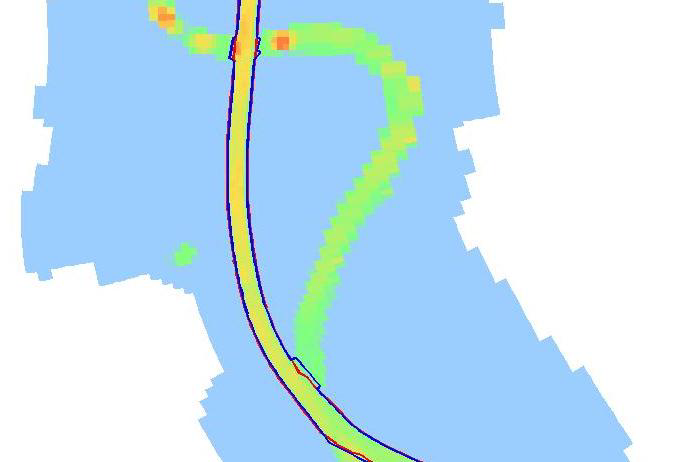
\includegraphics[width=\textwidth,height=7cm]{figures/Fig3-2.png}
\caption{Detection of bank lines at a shortcut in the Meuse river.
Red: Baseline 'section 1-2 boundary', Blue: detected bank line from WAQUA computation}
\label{Fig3.2}
\end{figure}

\begin{figure}[!hb]
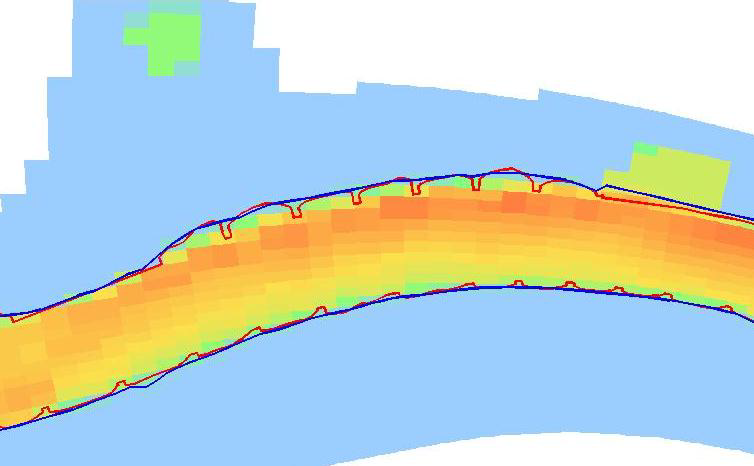
\includegraphics[width=\textwidth,height=7cm]{figures/Fig3-3.png}
\caption{Detection of a bank line close to groynes}
\label{Fig3.3}
\vspace{-0.75cm} 
\end{figure}
\clearpage

\section{Common issues with bank line detection} \label{Sec:DetectIssues}
It is advised to check the detected bank lines shown in the graphical output of the 'banklines' mode before continuing with the 'bankerosion' mode.
This section describes some common issues and their solutions.

\subsection{Detection of adjacent water body}
At some locations an adjacent water body is located within the given search distance from the predefined bank lines (parameter \command{Dlines}).
As a result the bank line of the adjacent water body is found, instead of the bank line of the main river channel.
As a result the initial bank line shows strange variations.
This is the case between kilometre 20 and 21 in \autoref{Fig_issue_bankline} location A.

\begin{figure}[!hb]
	\center
	\resizebox{15cm}{!}{
		\input{figures/detection_issue.pdf_tex}
	}
	\caption{Detection of the initial bank line close to adjacent water bodies}
	\label{Fig_issue_bankline}
\end{figure}

By decreasing the parameter \command{Dlines} you decrease the search distance from the predefined lines for determining the bank lines.
As a result, you decrease the chance that the bank line of an adjacent water  body is found.
However, you won't find a correct initial bank line if you make the parameter \command{Dlines} too small, this can be especially the case close to groins, at wide shallow areas or along banks with a relatively flat slope (see left bank between kilometre 22 and 23 in \autoref{Fig_issue_bankline} location B).

Another option is to edit the initial bank line manually by removing the points that fall in the adjacent water body, so only the points along the main channel remain.

\subsection{Irregularities in the detected bank line}
\autoref{Fig_issue_bankline} location C shows at the right outer bank after kilometre 22.5 a strange irregularity in the detected initial bank line.
This type of irregularities develop either by the detection of adjacent water body's, by the cut-off of connections with side channels (see \autoref{Fig_issue_bankline2}) or harbours or other irregularities along the bank.
It is advised to edit the initial bank line manually by removing some of the points so a smooth bank line along the main channel remains, because these irregularities influence the distance between the bank and the fairway and thus result in strange irregular patterns in wave heights and erosion along that bank.

\begin{figure}[!h]
	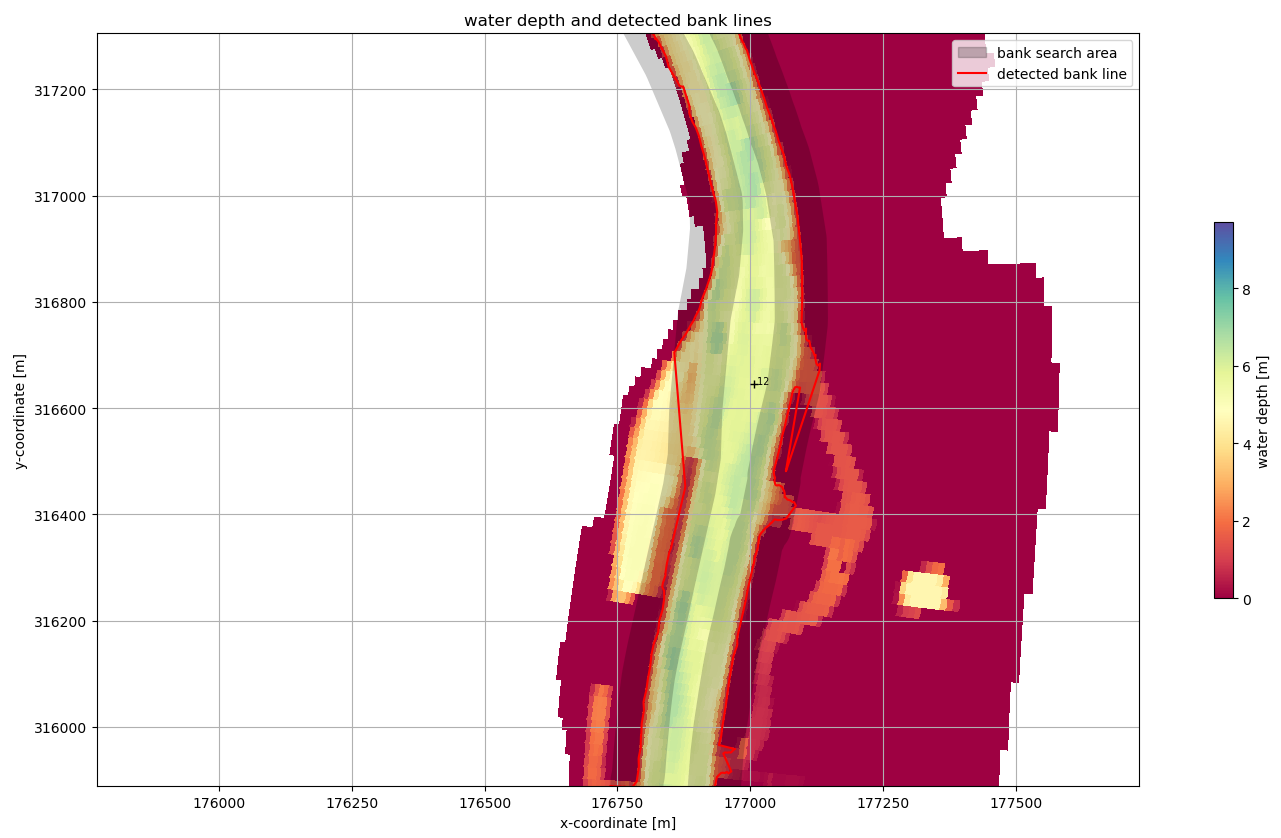
\includegraphics[width=\textwidth]{figures/detection_issue2.png}
	\caption{Detection of the initial bank line at the connection with a side channel}
	\label{Fig_issue_bankline2}
\end{figure}

\section{Shifting the bank lines} \label{Sec:BankShift}

The new location of the bank line is determined by shifting each bank line segment individually by its local erosion distance.
In the case of a concave bend the eroding segments move apart; a new bank segment is inserted connecting the two end points of the previously connected segments (see \autoref{Fig:erode_shift}, subplot a).
In case of a convex bend the eroding segments overlap; in this case the new bank line follows the outline of furthest erosion (see subplot b).

\begin{figure}[!h]
\center
\resizebox{12cm}{!}{
   \input{figures/erode_shift_step.pdf_tex}
}
\caption{Shifting a bank line first moves each line segment, and subsequently adds or removes segments as necessary}
\label{Fig:erode_shift}
\end{figure}

%\chapter{Potential bank line shift and bank erosion} \label{Chp4}

Wanneer de ligging van de initiele oeverlijn bekend is, kan de potentiele oeverlijnverschuiving en oeverafslag worden bepaald.
De ontwikkelde oevererosiemodule is bedoeld als hulpmiddel om de potentiele oevererosie in te kunnen schatten en niet om de daadwerkelijke oevererosie te voorspellen.
Binnen de oevererosiemodule worden twee erosiemechanismen meegenomen: erosie door scheepsgolven en erosie door stroming.
Deze mechanismen worden in de volgende twee paragrafen verder uitgewerkt.
Verder wordt in paragraaf 0 uitgelegd hoe de oeverlijnverschuiving in zijn werk gaat.
De bepaling van het potentieel geerodeerd volume wordt uitgewerkt in \autoref{Sec4.4}.
In \autoref{Sec4.5} wordt uitgelegd hoe er kan worden omgegaan met een variabel afvoerniveau.
Het bepalen van de evenwichtsoever en het daarbij behorende geerodeerde volume wordt uitgelegd in \autoref{Sec4.6}.
Ten slotte worden enkele van de beperkingen van de oevererosiemodule aangestipt in \autoref{Sec4.7}.

\section{Determining potential erosion by ship waves} \label{Sec4.1}

Scheepsgolven zijn een van de belangrijkste factoren wat betreft oeverafslag (Verheij (2000))  en worden daarom als eerste oevererosiemechanisme meegenomen in de oevererosiemodule.
 De afleiding voor de erosieformulering voor scheepsgolven is overgenomen uit de BEM module (Verheij (2000), Stolker \& Verheij (2001b)) en definities van grootheden zijn gegeven in \autoref{Fig4.1}.

\begin{figure}
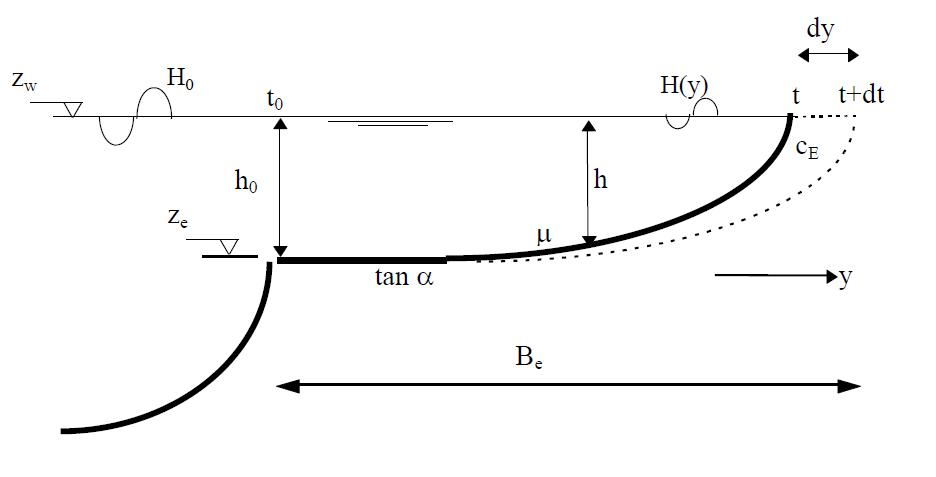
\includegraphics[width=8cm]{figures/Fig4-1.png}
\caption{Definities grootheden erosie door golven}
\label{Fig4.1}
\end{figure}

Op basis van grootschalige Deltagootproeven, waarbij diverse taluds van verschillende samenstelling werden belast onder loodrechte golfaanval, is afgeleid dat de erosiesnelheid kwadratisch toeneemt met de golfhoogte bij de oever:

\begin{equation}
\diff{y}{t} = c_E H^2
\label{Eq1.1}
\end{equation}

met:

\begin{symbollist}
\item[$y$] breedte van de afgekalfde oeverstrook \unitbrackets{m}
\item[$c_E$] sterkte coefficient voor oevermateriaal \unitbrackets{m\textsuperscript{-1}s\textsuperscript{-1}}
\item[$H$] golfhoogte bij de oever \unitbrackets{m}
\end{symbollist}

In het algemeen wordt verondersteld dat de afname van de golfhoogte via een negatieve e-macht is gerelateerd aan de breedte van de oeverstrook:

\begin{equation}
H = H_0 e^{-\mu y}
\label{Eq1.2}
\end{equation}

Hierin is:

\begin{symbollist}
\item[$H_0$] initiele golfhoogte aan het begin van de vooroever \unitbrackets{m}
\item[$\mu$] parameter voor golfdemping \unitbrackets{m\textsuperscript{-1}}
\end{symbollist}

Substitutie van \autoref{Eq1.2} in \autoref{Eq1.1} levert een differentiaalvergelijking op met de algemene oplossing:

\begin{equation}
\Delta n_\text{wave} = \frac{1}{2 \mu} ln ( 2 \mu c_E H_0^2 t + 1 )
\end{equation}

waarbij:

\begin{symbollist}
\item[$\Delta n_\text{wave}$] afstand waarmee de oeverlijn verschuift \unitbrackets{m}
\item[$t$] tijd \unitbrackets{s}
\end{symbollist}

Deze formule is toepasbaar voor zowel wind- als scheepsgolven.
In geval van scheepsgolven kan voor de tijd $t$ worden uitgegaan van de volgende relatie

\begin{equation}
t = T N n t_\text{eros} \text{ met } T = 0.51 \frac{v_s}{g} \text{.}
\end{equation}

waarbij:

\begin{symbollist}
\item[$T$] periode van de scheepsgolven \unitbrackets{s}
\item[$N$] aantal ongeladen schepen per jaar \unitbrackets{-}
\item[$n$] aantal golven per schip \textbf{-}
\item[$v_s$] vaarsnelheid schepen \unitbrackets{m/s}
\item[$g$] valversnelling 9.81 \unitbrackets{m/s\textsuperscript{2}}
\item[$t_\text{eros}$] beschouwde periode \unitbrackets{jaar}
\end{symbollist}

De waarde voor de initiele golfhoogte aan het begin van de vooroever $H_0$ kan met behulp van formules zoals uit DIPRO worden berekend aan de hand van het type maatgevende schepen, hun vaarsnelheid en diepgang, de afstand tussen de vaargeul en de oever en de waterdiepte (zie Bijlage A5A).

De parameter $\mu$ kan worden gebruikt om de invloed in rekening te brengen van de vorm van de vooroever op de golfdemping, maar ook het dempende effect van vooroeverconstructries, vegetaties, en afzettingen van oevermateriaal.
In de oevererosiemodule wordt alleen het effect van de helling van de vooroever op de golfdemping meegenomen.
De dempingsterm voor glooiende bodemhellingen wordt als volgt bepaald (Verheij (2000)):

\begin{equation}
\mu_\text{vo} = \frac{\tan \alpha}{H_0}
\end{equation}

Waarbij $\tan \alpha = \frac{1}{n}$ voor een vooroever met een helling van 1:$n$ (zie ook \autoref{Fig4.1}).
Uitgaande van een initiele golfhoogte $H_0 = 0.4$ leidt een helling tussen de 1:100 en 1:20 tot waarden van $\mu_\text{vo}$ liggend tussen 0.025 en 0.125.
In \autoref{Fig4.2} is een voorbeeld gegeven van de invloed van de dempingsparameter $\mu_\text{vo}$ op de oevererosie door golven.

\begin{figure}
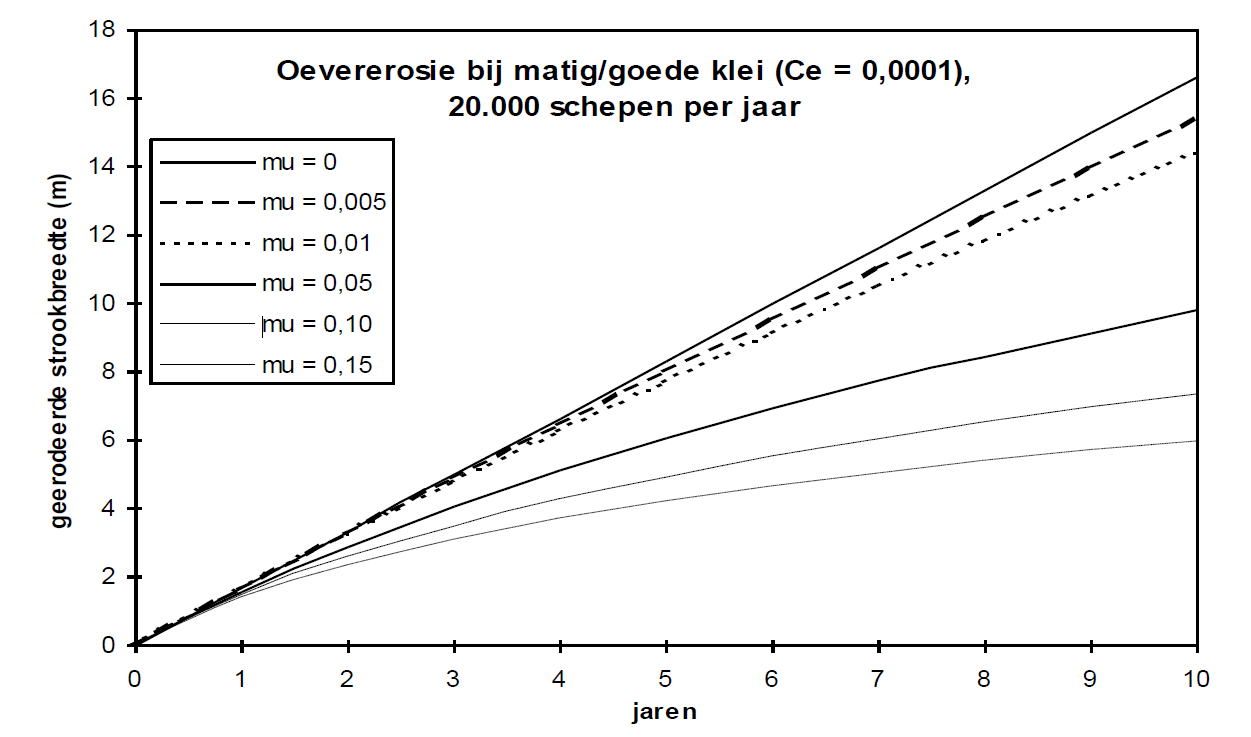
\includegraphics[width=\textwidth]{figures/Fig4-2.png}
\caption{Voorbeeld van oevererosie door golven voor matig/goede klei.}
\label{Fig4.2}
\end{figure}

Naast de golfdemping door de helling van de vooroever kunnen de inkomende golven ook worden gedempt door de begroeiing.
Voor golfdemping door riet is de volgende relatie beschikbaar

\begin{equation}
\mu_r = 8.5 \cdot 10^{-4} N_r^{0.8}
\end{equation}

met $N_r$ de rietstengeldichtheid (aantal stengels per vierkante meter).
De totale golfdemping door de helling van de vooroever en riet wordt dan

\begin{equation}
\mu_\text{tot} = \mu_\text{vo} + \mu_r
\end{equation}

De waarde voor de sterkte van het oevermateriaal $c_E$ hangt af van de samenstelling van de oever en kan ruimtelijk varieren.
Waarden voor $c_E$ voor verschillende oeversamenstellingen zijn te vinden in \autoref{Tab4.1}.
Per oeverlijn moet in een tekstbestand worden aangegeven uit welke klasse het oevermateriaal bestaat voor een bepaald riviertraject.

\begin{table}
\begin{tabular}{llll}
Klasse & Grond & $c_E$ \unitbrackets{m\textsuperscript{-1} s\textsuperscript{-1}} & $\tau_c$ \unitbrackets{Pa} \\ \hline
0 & Beschermde oeverlijn & 0 & $\infty$ \\
1 & Begroeide oeverlijn & 0.02 10\textsuperscript{-4} & 95 \\
2 & Goede klei & 0.6 10\textsuperscript{-4} & 3 \\
3 & Matig / slechte klei  & 2 10\textsuperscript{-4} & 0.95 \\
4 & Zand & 12.5 10\textsuperscript{-4} & 0.15 \\ \hline
\end{tabular}
\caption{Klassenindeling grondsoorten oevererosiemodule}
\label{Tab4.1}
\end{table}

\section{Determining potential erosion by currents} \label{Sec4.2}

Naast oeverafslag door scheepsgolven kan ook een sterke stroming langs de oever zelf zorgen voor oevererosie.
Dit mechanisme wordt ook meegenomen in de oevererosiemodule.
Voor elke oeverlijn kan de potentiele oevererosie door stroming bij een bepaalde afvoer $Q$ worden bepaald aan de hand van de volgende formule:

\begin{equation}
\Delta n_\text{flow} = E \left ( \frac{u_b^2}{u_c^2} - 1 \right ) t_\text{eros}
\end{equation}

met

\begin{symbollist}
\item[$\Delta n_\text{flow}$] afstand waarmee de oeverlijn verschuift in periode $t_\text{eros}$ \unitbrackets{m}
\item[$E$] erosiecoefficient van de oever \unitbrackets{m/s}
\item[$u_b$] stroomsnelheid langs de oeverlijn \unitbrackets{m/s}
\item[$u_c$] kritische stroomsnelheid voor erosie \unitbrackets{m/s}
\item[$t_\text{eros}$] beschouwde periode \unitbrackets{s}
\end{symbollist}

De erosiecoefficient wordt bepaald volgens:

\begin{equation}
E = \alpha \sqrt{\tau_c}
\end{equation}

met $\alpha$ = 2 10\textsuperscript{-7} \unitbrackets{m\textsuperscript{-3/2} kg\textsuperscript{1/2}} en $\tau_c$ \unitbrackets{N/m\textsuperscript{2}} de kritische schuifspanning voor erosie.
Deze waarde voor de erosiecoefficient is vergelijkbaar met erosiecoefficienten die in de literatuur gevonden worden (bijv.
Crosato, 2007).

Deze relatie tussen de kritische schuifspanning en de erosiecoefficient is echter niet universeel en daarom is het ook mogelijk om de erosiecoefficient als afzonderlijke invoer op te geven.

Voor de kritische stroomsnelheid voor erosie geldt:

\begin{equation}
u_c = \sqrt{\frac{\tau_c}{\rho} \frac{C^2}{g}}
\end{equation}

met $C$ \unitbrackets{m\textsuperscript{1/2}/s} de Chezy coefficient voor hydraulische ruwheid.
De waarde voor de Chezy coefficient wordt overgenomen uit de D-Flow FM berekening.

De stroomsnelheid langs de oever wordt bepaald aan de hand van de stroomsnelheid uit D-Flow FM.
De waarde voor de kritische schuifspanning voor erosie, $\tau_c$ , is gerelateerd aan de sterkte coefficient voor oevermateriaal, $c_E$ , zoals beschreven in Bijlage B)

\section{Total bank shift} \label{Sec4.3}

De totale oeverlijnverschuiving wordt gevonden door te sommeren over de oeverlijnverschuivingen veroorzaakt door de verschillende erosiemechanismen:

\begin{equation}
\Delta n = \Delta n_\text{flow} + \Delta n_\text{wave}
\end{equation}

De nieuwe locatie van een oeverlijn wordt bepaald door elk lijnsegment te verplaatsen volgens zijn lokale verschuiving.
De nieuwe locatie van een punt van de oeverlijn wordt gevonden door het snijpunt van de twee naburige segmenten te berekenen, zie \autoref{Fig4.3}.
Echter, in sommige situaties kan dit resulteren in erg grote verplaatsingen van punten, vooral wanneer naburige segmenten bijna in elkaars verlengde liggen.
In deze gevallen worden eerst twee locaties bepaald gebaseerd op de verplaatsing van elk van de naburige segmenten (rode stippen in \autoref{Fig4.4}).
De uiteindelijke locatie van een punt wordt dan bepaald door het gemiddelde van deze twee punten te nemen (groene stip in \autoref{Fig4.4}).


\begin{figure}
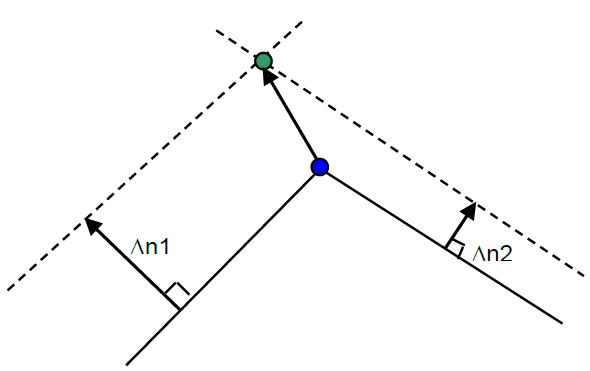
\includegraphics[width=6cm]{figures/Fig4-3.png}
\caption{Het verschuiven van een oeverlijn gebaseerd op het snijpunt van twee lijnsegmenten.
Blauw: oorspronkelijke locatie, Groen: nieuwe locatie}
\label{Fig4.3}
\end{figure}

\begin{figure}
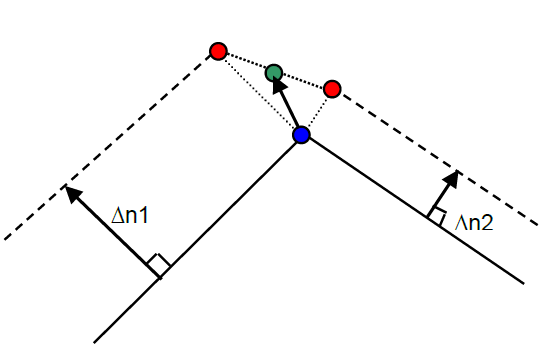
\includegraphics[width=5cm]{figures/Fig4-4.png}
\caption{Het verschuiven van een oeverlijn gebaseerd op de gemiddelde verplaatsing van twee lijnsegmenten.
Blauw: oorspronkelijke locatie, Rood: nieuwe locatie gebaseerd op individuele segmenten, Groen: nieuwe locatie (gemiddelde van de rode punten).}
\label{Fig4.4}
\end{figure}

Om numerieke problemen te voorkomen worden te kleine oeverlijnsegementen samengevoegd met hun buren.

\section{Potential bank erosion volume} \label{Sec4.4}

Naast de potentiele oeverlijnverschuiving is ook het potentiele volume aan sediment dat vrijkomt door erosie van belang.
Deze hoeveelheid sediment komt uiteindelijk in de rivier terecht, wat gevolgen kan hebben voor de bodemligging en eventueel noodzaak kan geven tot extra baggerwerkzaamheden.
Het potentiele volume aan sediment dat vrijkomt door erosie kan worden afgeschat door

\begin{equation}
V_\text{afslag} = ( \delta h_\text{bov} + \delta h_\text{ben} ) \Delta n
\end{equation}

waarbij $\Delta n$ de totale oeverlijnverschuiving en $\delta h$ het invloedsgebied van het afslagproces (boven en onder de waterspiegel).

Er wordt verondersteld dat de oever in zijn geheel terugschrijdt en daarom geldt voor het invloedsgebied boven de waterspiegel:

\begin{equation}
\delta h_\text{bov} = z_\text{oever} - z
\end{equation}

met

\begin{symbollist}
\item[$z$] waterspiegelniveau \unitbrackets{m}
\item[$z_\text{oever}$] niveau bovenkant steiloever \unitbrackets{m}
\end{symbollist}

De grootte van het invloedsgebied onder de waterspiegel wordt bepaald door de golfhoogte en het niveau tot waar het stortsteen blijft liggen.
Hiervoor wordt de volgende relatie gebruikt:

\begin{equation}
\delta h_\text{ben} = \min ( z-z_\text{ss}, 2 H )
\end{equation}

waarbij:

\begin{symbollist}
\item{$z$} waterspiegelniveau \unitbrackets{m}
\item{$z_\text{ss}$} niveau bovenkant stortsteen \unitbrackets{m}
\item{H} golfhoogte bij de oever \unitbrackets{m}
\end{symbollist}

In \autoref{Fig4.5} is geschematiseerd weergegeven wat het geerodeerd volume is voor verschillende situaties van de waterstand.


\begin{figure}
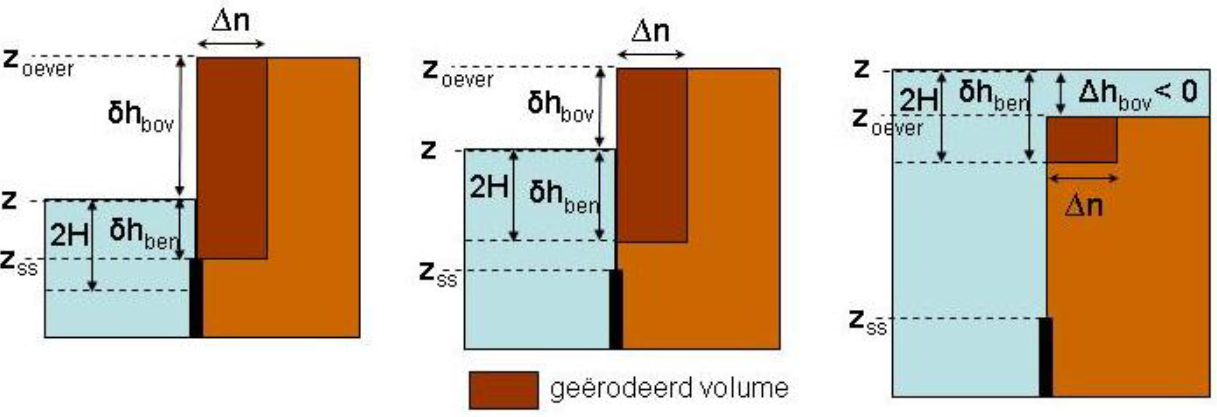
\includegraphics[width=\textwidth]{figures/Fig4-5.png}
\caption{Geerodeerd volume voor verschillende situaties van de waterstand.}
\label{Fig4.5}
\end{figure}

De terugschrijding van de oever wordt volledig bepaald door de oeverafslag, ongeacht of het materiaal dat voor de oever op de bodem terecht komt meteen wordt afgevoerd of niet.
Het afgeslagen materiaal beinvloedt wel de vervolgerosie, omdat het in zekere zin de oever beschermt.
De invloed hiervan kan niet worden bepaald door alleen een sedimentbalans op te stellen a.d.h.v.
een sedimenttransportformule, omdat soms grote hompen klei blijven liggen die eerst moeten desintegreren voordat de stroming ze kan meenemen.
De invloed van het afgeslagen materiaal op de golfhoogte (en daardoor de erosie door scheepsgolven) kan wel worden meegenomen door de parameter voor golfdemping, $\mu$, te verhogen.

\section{Variable discharge} \label{Sec4.5}

Het meenemen van een variabele afvoer is mogelijk door de afvoerverdeling te schematiseren met een hydrograaf.
Deze hydrograaf bestaat uit $n_Q$ afvoerniveaus en hun bijbehorende kans op voorkomen.
Voor elk afvoerniveau wordt een aparte D-Flow FM-berekening uitgevoerd.
Uit deze D-Flow FM simulaties kunnen dan de stroomsnelheid langs de oeverlijn en het niveau van de waterspiegel worden afgeleid.
Hierbij wordt er vanuit gegaan dat in ieder geval de afvoer wordt meegenomen die is gebruikt om de initiele oeverlijn te bepalen (de gemiddelde afvoer).

Vervolgens worden oeverlijnverschuivingingen voor de afzonderlijke afvoerniveaus bepaald en deze worden daarna gewogen gesommeerd aan de hand van de kans van voorkomen van het betreffende afvoerniveau.
Voor elk afvoerniveau $Q_i$ wordt dus eerst de totale erosie $\Delta n ( Q_i )$ voor die afvoer bepaald, die bestaat uit een deel veroorzaakt door scheepsgolven en een deel veroorzaakt door stroming.

Een variabele afvoer betekent dat ook het niveau van de waterspiegel tijdsafhankelijk is en daarmee de locatie waar de oevererosie optreedt.
In de oevererosiemodule wordt echter uitgegaan van een initiele oeverlijn (behorende bij een gemiddelde afvoer).
De mate van erosie van deze lijn varieert echter wel met de afvoer.


\subsection{Erosion by ship waves}

Een varierend afvoerniveau zorgt voor een varierend niveau van de waterspiegel.
De initiele oeverlijn is echter alleen onderhevig aan erosie door golven bij een gegeven afvoer $Q_i$ als de hoogte van de lijn in het invloedsgebied [$z(Q_i) - 2 H$, $z(Q_i) + \frac{1}{2} H$] ligt, waarbij $H$ de golfhoogte bij de oever en $z(Q_i)$ het niveau van de waterspiegel bij afvoer $Q_i$.
In de voorbeelden weergegeven in \autoref{Fig4.6} is de oeverlijn dus alleen onderhevig aan erosie door golven bij afvoerniveaus $Q_2$ en $Q_3$.
Of een oeverlijn binnen het invloedsgebied ligt waarin erosie door golven moet worden meegenomen, kan plaatsafhankelijk zijn.
In het benedenstroomse gebied liggen de waterniveaus bij verschillende afvoeren in het algemeen dichter bij elkaar dan bovenstrooms en ook vlakbij een stuw met een opgegeven stuwpeil kan het waterniveau redelijk constant blijven voor verschillende afvoeren.

\begin{figure}
\begin{tabular}{p{6cm}p{6cm}}
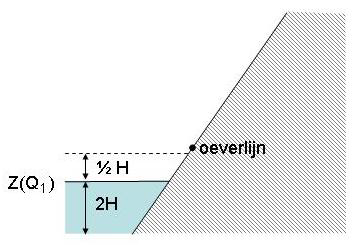
\includegraphics[width=5cm]{figures/Fig4-6a.png} \linebreak
a) &
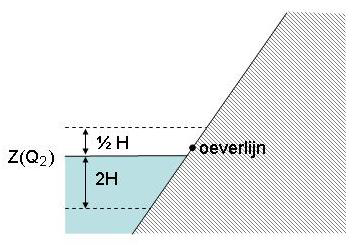
\includegraphics[width=5cm]{figures/Fig4-6b.png} \linebreak
b) \\
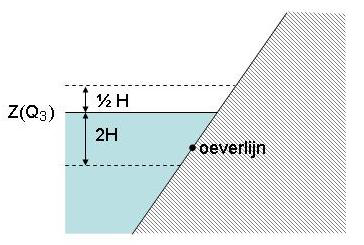
\includegraphics[width=5cm]{figures/Fig4-6c.png} \linebreak
c) &
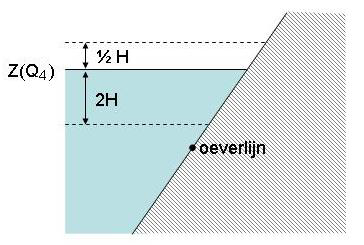
\includegraphics[width=5cm]{figures/Fig4-6d.png} \linebreak
d) \\
\end{tabular}
\caption{Erosie door golven bij meerdere afvoerniveaus: a) geen erosie, oeverlijn ligt boven invloedsgebied b) erosie, c) erosie, d) geen erosie, oeverlijn ligt onder invloedsgebied}
\label{Fig4.6}
\end{figure}

\subsection{Erosion by currents}

Voor elk afvoerniveau wordt de erosie door stroming bepaald met behulp van de stroomsnelheid langs de oeverlijn behorende bij het betreffende afvoerniveau.
Hierbij is er natuurlijk alleen stroming langs de oeverlijn als deze lijn op of onder de waterspiegel ligt.
In de voorbeelden weergegeven in \autoref{Fig4.6} is de oeverlijn dus alleen onderhevig aan erosie door stroming bij afvoerniveaus $Q_3$ en $Q_4$.

\subsection{Total erosion}

De totale verschuiving van de oeverlijn bij het meenemen van meerdere afvoerniveaus wordt gevonden door de oeverlijnverschuivingen bij de verschillende afvoeren gewogen te sommeren over alle afvoerniveaus:

\begin{align}
\Delta n_\text{tot} &= \sum_{i=1}^{n_Q} p(Q_i) \Delta n(Q_i) \\
                    &= \sum_{i=1}^{n_Q} p(Q_i) \left [ \Delta n_\text{wave}(Q_i) + \Delta n_\text{flow}(Q_i) \right ]
\label{Eq1.3}
\end{align}

waarbij:

\begin{symbollist}
\item[$\Delta n_\text{tot}$]  totale verschuiving van de oeverlijn \unitbrackets{m}
\item[$n_Q$] aantal gebruikte afvoerniveaus \unitbrackets{-}
\item[$p(Q_i)$] jaarlijkse kans op afvoer $Q_i$ \unitbrackets{-}
\item[$\Delta n(Q_i)$] totale verschuiving van de oeverlijn bij afvoer $Q_i$ \unitbrackets{m}
\item[$\Delta n_\text{wave}(Q_i)$] verschuiving van de oeverlijn door scheepsgolven bij afvoer $Q_i$ \unitbrackets{m}
\item[$\Delta n_text{flow}(Q_i)$] verschuiving van de oeverlijn door stroming bij afvoer $Q_i$ \unitbrackets{m}
\end{symbollist}

De verschuiving van de oeverlijn kan dan weer op dezelfde manier worden bepaald als uitgewerkt in paragraaf 0, maar nu met de totale oeverlijnverschuiving zoals gegeven in \autoref{Eq1.3}.
De potentiele oeverafslag dient eerst per afvoerniveau te worden berekend (zie \autoref{Sec4.4}).
Daarna kan de totale potentiele oeverafslag worden bepaald door gewogen te sommeren met de kans van voorkomen van het betreffende afvoerniveau, analoog aan de bepaling van de totale oeverlijnverschuiving (\autoref{Eq1.3}).

\section{Determining equilibrium bank} \label{Sec4.6}

In van der Mark (2011), Hoofdstuk 3 is een analyse gemaakt van kentallen voor te verwachten oevererosie langs de IJssel.
Daarin wordt gesteld dat de meest waarschijnlijke te verwachten taludhelling van de evenwichtsoever 1:20 is.
Aan de hand hiervan kan een schatting worden gegeven van de erosieafstand $\Delta n_\text{eq}$ voor het behalen van de evenwichtssituatie (zie ook \autoref{Fig4.7}):

\begin{equation}
\Delta n_\text{eq} = \frac{h_t}{\mu_\text{slope}}
\end{equation}

Waarbij $\mu_\text{slope}$ de inverse van de taludhelling van de evenwichtsoever (default waarde 1/20) en $h_t = \max (z_\text{up} - z_\text{do}, 0)$ met $z_\text{up} = \min [ h_\text{bank}, z(Q_\text{ref}) + 2 H_0]$ en $z_\text{do} = \max [ z_\text{ss}, z(Q_\text{ref}) - 2 H_0 ]$.
Het totaal afgeslagen volume voor het bereiken van een evenwichtsoever is dan gelijk aan

\begin{equation}
V_\text{eq} = ( \frac{1}{2} h_t + h_s ) \Delta n_\text{eq}
\end{equation}

met $h_s = \max [ h_\text{bank} - z(Q_\text{ref}) _ 2 H_0, 0 ]$.


\begin{figure}
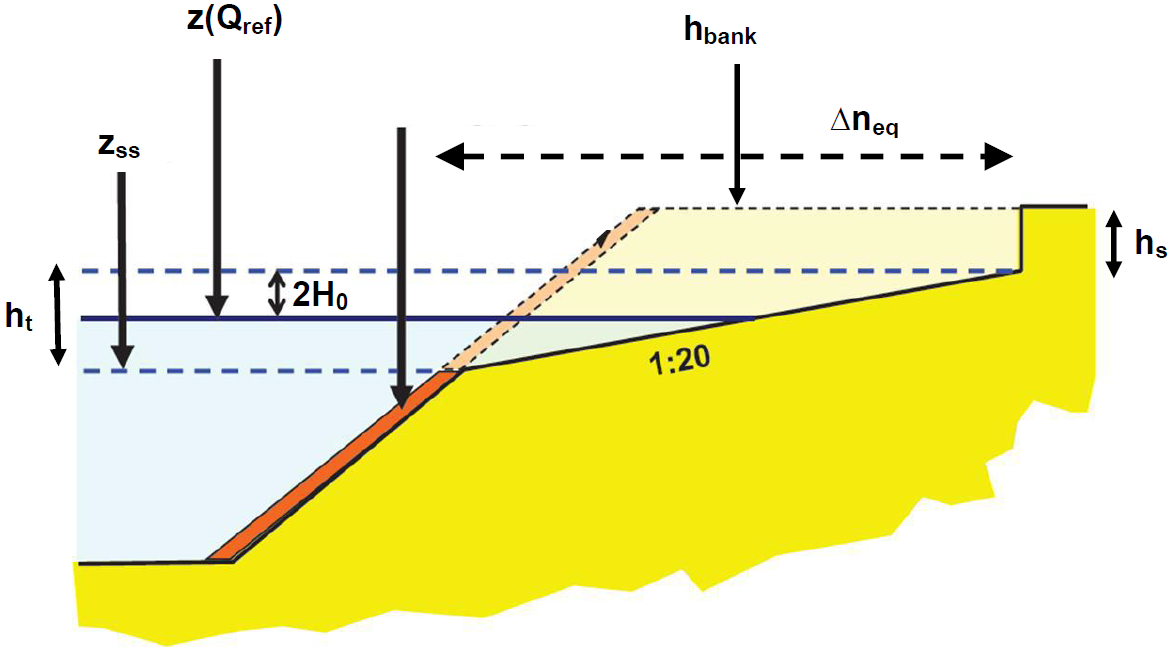
\includegraphics[width=\textwidth]{figures/Fig4-7.png}
\caption{Geschatte profiel evenwichtsoever.}
\label{Fig4.7}
\end{figure}

\section{Limitations of D-FAST Bank Erosion} \label{Sec4.7}

De oevererosiemodule is bedoeld als hulpmiddel om in te kunnen schatten waar potentieel oevererosie plaats kan vinden en niet om de daadwerkelijke oevererosie te voorspellen.
In deze sectie worden een paar beperkingen van de oevererosiemodule aangestipt.

\subsection{Homogeneous bank}

Een van de belangrijkste beperkingen is dat de samenstelling van de oever homogeen wordt verondersteld.
Dit is in de werkelijkheid niet het geval.
Er worden vaak horizontale of verticale lagen waargenomen.
In \autoref{Fig4.8} worden beide situaties weergegeven en de manier waarop het erosieproces plaatsvindt in het geval van horizontale lagen.
Om verticale lagen te kunnen modelleren, kunnen verschillende waarden van $c_E$ worden gebruikt voor elke laag.
De situatie met horizontale lagen is complexer, omdat in dit geval plotseling grote hoeveelheden oevermateriaal in een keer naar beneden kunnen glijden.

\begin{figure}
\begin{tabular}{p{6cm}p{6cm}}
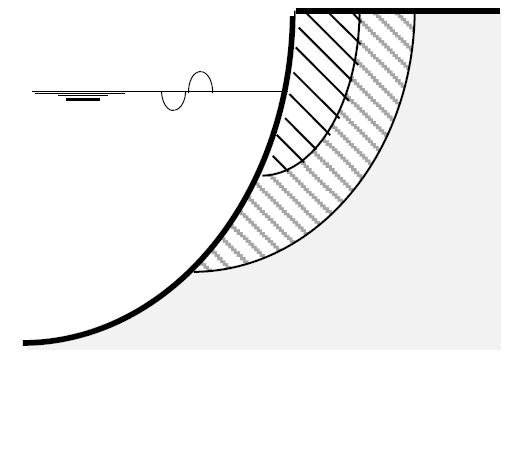
\includegraphics[width=5cm]{figures/Fig4-8a.png} \linebreak
a) vertical layers &
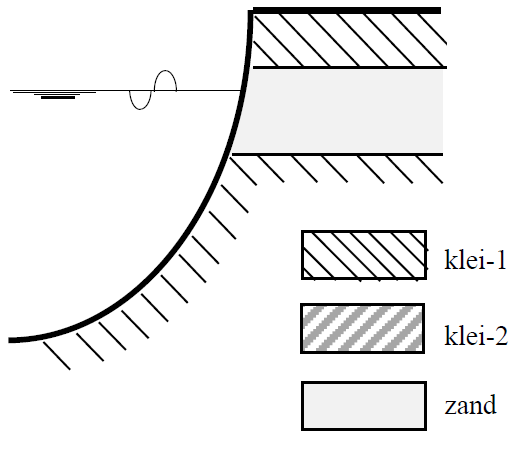
\includegraphics[width=5cm]{figures/Fig4-8b.png} \linebreak
b) horizontal layers \\
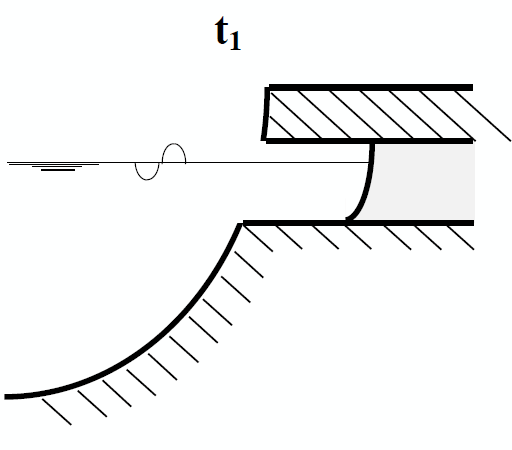
\includegraphics[width=5cm]{figures/Fig4-8c.png} \linebreak
c) erosion process in case of horizontal layers &
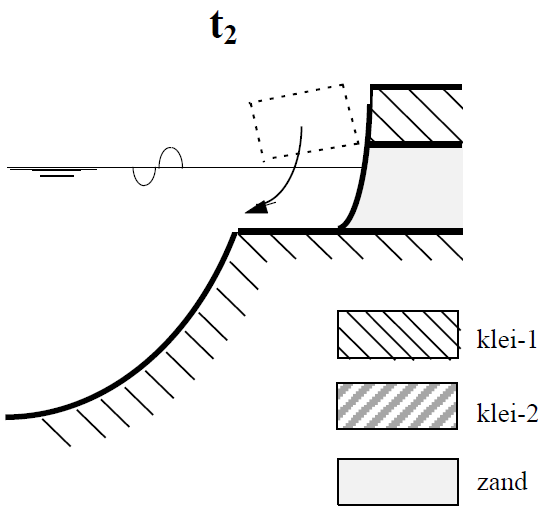
\includegraphics[width=5cm]{figures/Fig4-8d.png} \\
\end{tabular}
\caption{Non-homogeneous banks.}
\label{Fig4.8}
\end{figure}

\subsection{Only erosion along initial bank line}

Er wordt alleen oevererosie bepaald voor de opgegeven initiele oeverlijn (behorende bij een gemiddelde afvoer).
In werkelijkheid is het echter ook mogelijk dat er oevererosie op andere locaties plaatsvindt.

\subsection{Only erosion by ship waves and currents}

In de oevererosiemodule wordt alleen erosie door scheepsgolven en stroming gemodelleerd.
Andere erosiemechanismen zoals windgolven, uitstromend grondwater, bevriezing en vertrapping door vee worden in de module niet meegenomen.

\subsection{Profile and bed level remain constant}

Door oevererosie verandert lokaal de breedte van de rivier en ook zorgt het afgeslagen materiaal voor een andere bodemligging.
Hierdoor veranderen ook de stromingscondities in de rivier en langs de oever.
Aangezien de oevererosiemodule is gebaseerd uitkomsten van D-Flow FM berekeningen wordt deze dynamiek van de bodem en oevers echter niet meegenomen.


%\nonumchapter{References}
%Crosato, A. (2007), Effects of smoothing and regridding in numerical meander migration models. Water Resources Research, Vol 43.

CUR, (1996). Erosie van onverdedigde oevers, CUR-rapport 96-7, Gouda.

IWACO, Waterloopkundig Laboratorium en CSO (1998). Trajectnota/MER Zandmaas-Maasroute, Ontwerp natuurvriendelijke oevers. eindrapport 3361070.

Mark, R. van der, R.A.M. van der Sligte, A. Becker, E. Mosselman \& H.J. Verheij (2011), Morfologische effectstudie KRW-maatregelen IJssel.
Rapport 1204885, Deltares, Delft.

Schuurman, F. (2010), Casestudie oevererosie Maas, DHV memo kenmerk LW-AF20100800/RK, 30 december 2010.

Sieben, J., J.A.F. van Essen, M.J.M. Scholten and L.W.J. van Hal, (2005), Inschatting van de kans op achterloopsheid bij kribben, RIZA werkdocument 2005.148x.

Sieben, J. (2005), Wie het water deert, die het water keert - Inventarisatie van beheer en onderhoud van kribben en oeververdedigingen, RIZA werkdocument 2005.034x.

Spruyt, A. (2009), Shifting margins, behaviour of dynamic banks, Internal memorandum 200186-003-ZWS-0003-v2-m-Oeverdetectie, Deltares, Delft, 4 november 2010.

Spruyt, A. \& E. Mosselman (2010), Deelproject 3: Schuivende marges, gedrag van dynamische oevers (Shifting margins, behaviour of dynamic banks).
Appendix C in TO Rivierkundige Onderzoeksthema's; Rapportage 2009, Rapport 1200186.000, Deltares.

Stolker, C. \& H.J. Verheij (2001a), Gevoeligheidsonderzoek sedimentatie en erosie in kribvakken langs de Lek. Rapport Q2792, WL | Delft Hydraulics, Delft, Februari 2001.

Stolker, C. \& H.J. Verheij (2001b), Calibratie van een oeverafslagmodel voor de Zandmaas. Rapport Q3060, WL | Delft Hydraulics, Delft, November 2001.

TAW (1998), Technisch rapport erosiebestendigheid van grasland als dijkbekleding, Technische Adviescommissie voor de Waterkeringen, Delft.

Verheij, H.J., Meijer, D.G., Kruse, G.A.M., Smith, G.M., Vesseur, M., (1995). Investigation of the strength of a grass cover upon river dikes [in Dutch], Report Q1878, Deltares, Delft.

Verheij, H.J. (2000), Samenwerkingsproject Modellering Afslagoevers. Rapport Q2529, WL | Delft Hydraulics, Delft.

Verheij, H.J., F. van der Knaap \& H. Sessink (2007), Verder ontwikkelen van oeverafslagmodel BEM. Rapport Q4264.02, WL | Delft Hydraulics, Delft.

Vroeg, J.H. de (1999), Breach growth in cohesive materials : selection of cases. Rapport H3468, WL | Delft Hydraulics, Delft.

%\bibliography{../common/deltares_manual}

%\appendix
%\chapter{Bank strength coefficients for different soil types} \label{bankcomp}

The strength coefficient of the bank material, $c_E$ , and the critical shear stress for erosion, $\tau_c$, for different soil types are given in \autoref{Tab5.1} based on \citep{VerheijMKSV95, Vergeer96, VerheijKNS98, Vroeg99}.

The following relation can be used

\begin{equation}
c_E = \frac{\beta}{\tau_c}
\end{equation}

where $\beta$ = $1.85 \cdot 10^{-4}$ \unitbrackets{kg / (m\textsuperscript{2} s\textsuperscript{3})}.

\begin{table}[H]
\center
\begin{tabular}{p{5cm}rr}
Bank type & $c_E$ \unitbrackets{m\textsuperscript{-1}s\textsuperscript{-1}} & $\tau_c$ \unitbrackets{Pa} \\ \hline
Protected bank & 0 & $\infty$ \\
Sturdy grass & 0,01 $10^{-4}$ & 185 \\
Mediocre grass & 0,02 $10^{-4}$ & 93 \\
Bad grass & 0,03 $10^{-4}$ & 62 \\
Very good clay (compact) & 0,5 $10^{-4}$ & 4 \\
Clay with 60\% sand (firm) & 0,6 $10^{-4}$ & 2,5 \\
Good clay with  little structure & 0,75 $10^{-4}$ & 2 \\
Strongly structure good clay (mediocre) & 1,5 $10^{-4}$ & 1,5 \\
Bad clay (weak) & 3,5 $10^{-4}$ & 0,65 \\
Sand with 17\% silt & 10 $10^{-4}$ & 0,20 \\
Sand with 10\% silt & 12,5 $10^{-4}$ & 0,15 \\
Sand with 0\% silt & 15 $10^{-4}$ & 0,10 \\ \hline
\end{tabular}
\caption{Corresponding values for $c_E$ and $\tau_c$ \citep{VerheijMKSV95}.}
\label{Tab5.1}
\end{table}

%\chapter{Determining ship induced wave height at the beginning of the fore shore} \label{Chp:shipwaves}

To determine the ship induced wave height $H_0$ \unitbrackets{m} at the beginning of the fore shore, the following formula is used (source: Handleiding DIPRO, 1997)

\begin{equation}
H_0 = \alpha_1 h \left ( \frac{s}{h} \right )^{-1/3} Fr^4
\end{equation}

with

\begin{symbollist}
\item[$\alpha_1$] ship dependent coefficient \unitbrackets{-}
\item[$Fr$] Froude number ($Fr$<0.8) \unitbrackets{-}
\item[$h$] water depth (considering a  trapezoidal profile) \unitbrackets{m}
\item[$s$] distance of shore to ship \unitbrackets{m}
\end{symbollist}

The Froude number is computed according to:

\begin{equation}
Fr = \frac{v_s}{\sqrt{g h}}
\end{equation}

with

\begin{symbollist}
\item[$g$] gravity acceleration 9.81 \unitbrackets{m/s\textsuperscript{2}}
\item[$v_s$] ship velocity \unitbrackets{m/s}
\end{symbollist}

The value of the Froude number is limited to 0.8.

For the coefficient $\alpha_1$ the following values are used, with $T_s$ \unitbrackets{m} the draught of the ships:

\begin{tabular}{ll}
Ship type & $\alpha_1$ \\ \hline
Push barge & 0.5 \\
RHK ship / Motorship & 0.28 $T_s^\text{1.25}$ \\
Towboat & 1.0 \\ \hline
\end{tabular}

By using this formulas, the value of $H_0$ can be computed based on the dominant ship type, their velocity and draught, the distance between fairway and shore and the water depth.

To prevent wave load on smaller channels far from the main channel, the wave height is smoothly reduced to zero from distance $s_1$ to $s_0$ from the fairway.
This is accomplished by multiplying $H_0$ with the following function:

\begin{equation}
f(s) = \left \{ \begin{matrix}
1 & 0 < s < s_1 \\
\cos \left ( \frac{s - s_1}{s_0 - s_1} \pi \right ) & s_1 < s < s_0 \\
0 & s > s_0
\end{matrix} \right .
\end{equation}

The value for $s_0$ will be in the order of 150 - 200 m and for  the following relation is used: $s_1 = s_0 - 50$.
In \autoref{Fig5.1} the wave height $H_0$ as function of the distance from the fairway $s$ is depicted for various values of the water depth $h$ for a moter ship with a draught of 1.2 m with a relative velocity of $v_s = 6$ m/s.
The wave height is reduced to zero between $s_1 = 100$ m and $s_0 = 150$ m.

\begin{figure}
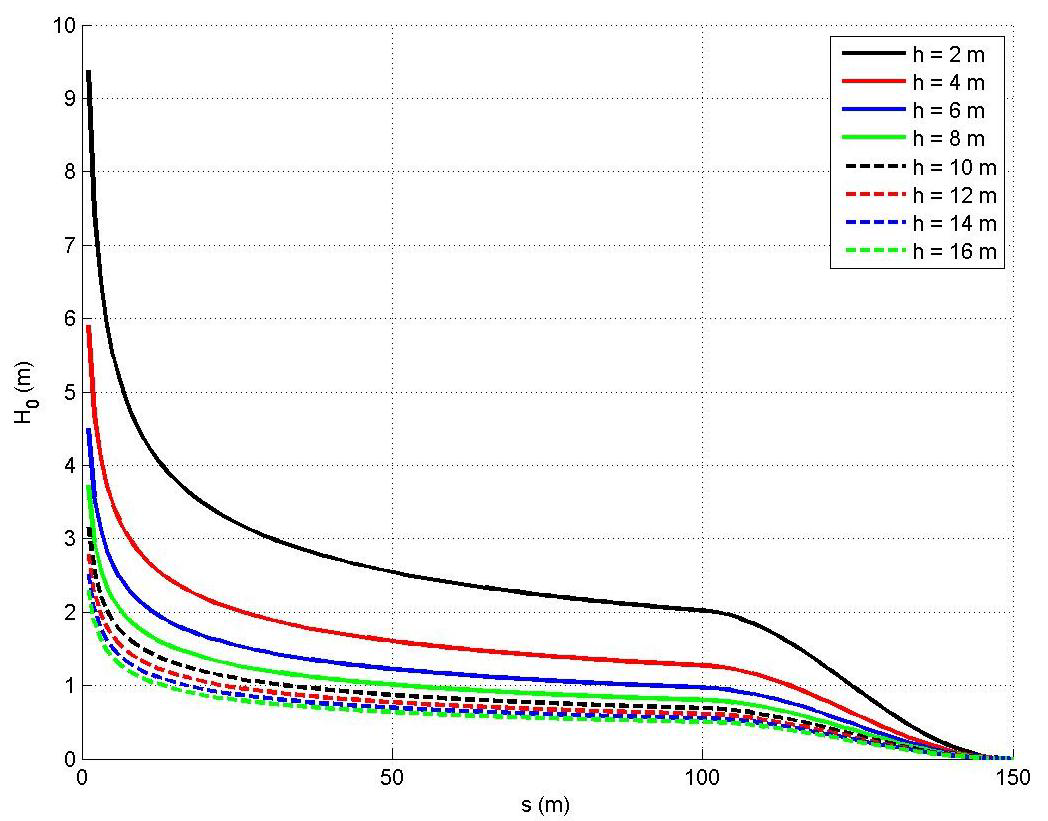
\includegraphics[width=\textwidth]{figures/Fig5-1.png}
\caption{Wave height as function from the distance from the fairway for different values of the water depth.}
\label{Fig5.1}
\end{figure}

%\chapter{Technical Reference Manual}
\markdownInput{techref.md}

%\pagestyle{empty}
%\cleardoublepage
%\mbox{}
%\includepdf[pages=2, offset=-72 -70]{cover/d-fast-bank-erosion.pdf} % links-rechts past precies
\end{document}
